\label{sect:sota_circulations}
Cette partie a pour objectif de recenser les projets valorisant des archives textuelles ou audiovisuelles,  avec un focus sur le développement d'outils numériques permettant d'identifier les différents formes de circulations culturelle ou intellectuelle. Nous y présentons des projets menés au sein d'institutions patrimoniales et académiques, avant d'aborder les évènements et revues spécialisés sur la question des circulations.
\section{Principaux acteurs}
\label{sect:sota_acteurs} Incontestablement, l'époque actuelle est profondément marquée par le \og{}déluge des données\fg{}, phénomène représentatif de la quatrième paradigme de la science, selon Jim Gray \citep[p.~30]{hey2009jim}. Ce nouveau paradigme scientifique s'appuie sur la capacité des ordinateurs de recueillir, stocker et analyser rapidement d'importants volumes de données. Par conséquent, les projets numériques sont aujourd'hui largement \og{}pilotés par les données (angl. \textit{data-driven})\fg{}\footnote{Ce terme fut introduit par \citet{Johns1991ShouldYB}, dans l'expression \textit{data-driven learning}.}, et ceux qui sont centrés sur les explorations des circulations culturelles au prisme du numérique se concrétisent à grande échelle. Les méthodes computationnelles des circulations ne se limitent pas à la gestion de corpus volumineux selon une perspective spatio-temporelle ; elles permettent également de dépasser les cadres nationaux, de remettre en question les hiérarchies entre objets d’étude, et ainsi de s'affranchir des \og{}réflexes nationalisateurs\fg{} et des \og{}jugements de valeur\fg{} souvent présents dans l'analyse des circulations culturelles \citep[p.~12]{joyeux2022circulations}.
%Les humanités numériques au service de l'analyse des circulations culturelles se manifestent sous forme de divers projets de recherche au niveau académique. 
Cette thématique est au c\oe{}ur des préoccupations des structures de recherche (laboratoires, chaires, équipes-projet), des évènements scientifiques ou même des numéros de revues spécialisés.

En France, plusieurs équipes de recherche académique constituent un environnement dynamique consacré à l'étude des phénomènes de circulation. L'équipe-projet \textsc{ObTIC} de Sorbonne Université, avec le projet \textsc{ModERN}, a pour objectif d'identifier et analyser des réseaux conceptuels et intertextuels sur une collection de textes des XVIII\ieme{} et XIX\ieme{} siècles. Au sein du même projet, nous notons les travaux de \citet{roe2023enlightenment} qui portent sur la détection de réemplois textuels à grande échelle et l'analyse de réseaux pour identifier les \og{}influenceurs\fg{} dans les ouvrages français du siècle des Lumières.
D'autres universités françaises, telles que l'École normale supérieure (\textsc{ENS-PSL}), ont développé certains projets ayant pour l'objectif la valorisation des archives philosophiques au prisme des humanités numériques. Le projet \og{}Nietzsche et son temps\fg{} analyse la genèse des concepts et des thèmes principaux de la philosophie de Nietzsche à travers l'édition et à l’interprétation de son \oe{}uvre avec des méthodes génétiques. De manière similaire, le projet \og{}DERRIDA HEXADÉCIMAL\fg{} s'est attaché à identifier les caractéristiques de l'invention scripturale propre à Derrida, en s'intéressant notamment à sa créativité linguistique (création de néologismes, mots-valise, jeux de signifiant,$\dots$), ainsi qu'à l'élaboration des concepts, en mobilisant pour cela des méthodes issues de la criminalistique numérique. Pour ce qui est du projet \og{}Foucault Fiches de lecture\fg{}, il vise d'une part à rendre accessibles les sources utilisées par le philosophe, et d'autre part à contribuer à l'élaboration d'une herméneutique philosophique, fondée sur l'étude de ses pratiques documentaires et de ses modes de travail.

À ces initiatives académiques s'ajoutent les travaux menés par la chaire des humanités numériques de l'université de Genève, qui s'articulent autour d'au moins trois projets : \textit{Artl@s}, \textit{Katabase -- Manuscripts Sales CatalogueS (MSS)} et \textit{Visual Contagions}. Le projet \textit{Artl@s} vise à cartographier la circulation mondiale des \oe{}uvres d'art à partir des documents textuels, notamment les catalogues d'expositions. \textit{Katabase -- MSS}, quant à lui, explore la circulation des manuscrits en tant que nouvelle perspective pour analyser la réception des auteurs et, par conséquent, les évolutions du canon littéraire. À la différence de ces deux projets fondés sur l'exploitation des sources textuelles, \textit{Visual Contagions} se penche sur la circulation mondiale des images à l'ère de l'imprimé, de 1890 jusqu'aux débuts d'Internet. Le tableau \ref{tab:equipes} résume les projets cités. 
% \ref{tab:events} et \ref{tab:revues}.

\begin{table}[htbp]
	\centering
	\renewcommand{\arraystretch}{1.5}
	\resizebox{\textwidth}{!}{%
		\begin{tabular}[t]{|p{7cm}|p{7cm}|}
			\hline
			\textbf{Équipe} & \textbf{Projets numériques des circulations} \\ \hline
			\begin{minipage}[t]{\linewidth}
				Équipe-projet \textsc{ObTIC}\\
				Sorbonne Université\footnote{\url{https://obtic.sorbonne-universite.fr/projets/}}\\
				Responsable : Glenn Roe
			\end{minipage}
			&
			\begin{minipage}[t]{\linewidth}
				\begin{itemize}[leftmargin=*]
					\item \textit{Mod\textsc{ERN}}\footnote{\url{https://modern.huma-num.fr/about/}} (2022-)
					
				\end{itemize}
			\end{minipage} \\ \hline
			\begin{minipage}[t]{\linewidth}
				Chaire des humanités numériques\\
				Université de Genève\footnote{\url{https://www.unige.ch/lettres/humanites-numeriques/recherche/projets}}\\
				Responsable : Béatrice Joyeux-Prunel
			\end{minipage}
			&
			\begin{minipage}[t]{\linewidth}
				\begin{itemize}[leftmargin=*]
					\item \textit{Artl@s}\footnote{\url{https://artlas.huma-num.fr/fr/}} (2009-)
					\item \textit{Katabase -- Manuscripts Sales CatalogueS (MSS)}\footnote{\url{https://katabase.huma-num.fr/}} (2020-) 
					\item \textit{Visual Contagions}\footnote{\url{https://www.unige.ch/visualcontagions/}} (2021-2024)
					
				\end{itemize}
			\end{minipage} \\ \hline
			\begin{minipage}[t]{\linewidth}
				Observatoire des humanités numériques\footnote{\url{https://odhn.ens.psl.eu/}.}\\
				École normale supérieure | \textsc{PSL}\\
				Responsable : Léa  Saint-Raymond
			\end{minipage} 
			& 
			\begin{minipage}[t]{\linewidth}
				\begin{itemize}[leftmargin=*]
					\item \og{}Nietzsche et son temps\fg{}\footnote{\url{http://www.item.ens.fr/nietzsche/}} (2009-)
					\item \og{}Foucault Fiches de Lecture \fg{}\footnote{\url{https://eman-archives.org/Foucault-fiches/}} (2013-)
					\item \og{}DERRIDA HEXADÉCIMAL\fg{}\footnote{\url{http://www.item.ens.fr/derrida-hexadecimal/}} (2018-2024)
				\end{itemize}
			\end{minipage} \\ \hline
		\end{tabular}%
	}
	\caption{Structures de recherche axées sur la thématique des circulations des savoirs.}
	\label{tab:equipes}
\end{table}





%
\begin{table}[htbp]
	\centering
	\resizebox{\textwidth}{!}{%
		\renewcommand{\arraystretch}{1.5}
		\begin{tabular}[t]{|p{3.5cm}|p{1.2cm}|p{5cm}|p{6cm}|}
			\hline
			\textbf{Type d'évènement} & \textbf{Année} & \textbf{Nom d'évènement} & \textbf{Thématiques} \\ \hline
			Colloque & 2025 &
			\begin{minipage}[t]{\linewidth}\og{}Le texte de l'autre. Dialogue interdisciplinaire autour de l'intertextualité et du discours rapporté\fg{}\footnote{\url{https://www.fabula.org/actualites/122618/le-texte-de-l-autre-dialogue-interdisciplinaire-autour-de-l-intertextualite-et-du-discours-rapporte.html}}
			\end{minipage}
			& Dialogues historiques des textes et des idées :
			\begin{itemize}
				\item études littéraires et historiques qui fondent leur existence sur la citation, l’évocation et l’analyse de textes antérieurs, sources premières de leurs réflexions
				\item études de l’histoire intellectuelle, l’histoire de l’éducation ou l’histoire religieuse, pour qui l’établissement de réseaux de citation(s) peut révéler la circulation d’idées, leur rejet ou leur acceptation
			\end{itemize} \\ \hline
			Colloque & 2023 &
			\begin{minipage}[t]{\linewidth}Humanistica 2023 \footnote{\url{https://humanistica2023.sciencesconf.org/}}
			\end{minipage}
			& \begin{itemize}
				\item migrations, mondialisation, transferts culturels, histoire transnationale
				\item histoire des objets
				\item circulations de motifs littéraires, visuels, sonores
				\item réemplois / emprunts / citations
			\end{itemize} \\ \hline
			Colloque & 2023 &
			\begin{minipage}[t]{\linewidth}\og{}De la transformation des sciences humaines par les humanités numériques\fg{} (ACFAS 2023)\footnote{\url{https://www.crihn.org/nouvelles/2022/12/11/colloque-de-la-transformation-des-sciences-humaines-par-les-humanites-numeriques-acfas-2023/}}
			\end{minipage} & 
			\begin{itemize}
				\item formes de production, circulation et validation des connaissances à l’époque du numérique dans le domaine des sciences humaines
			\end{itemize} \\ \hline
			Journée d'étude & 2021 &
			\begin{minipage}[t]{\linewidth}
				\og{}Circulation des écrits littéraires de la première modernité et humanités numériques\fg{}\footnote{\url{https://www.fabula.org/actualites/86846/circulation-des-ecrits-litteraires-de-la-premiere-modernite-et-humanites-numeriques.html}}
			\end{minipage}
			&
			\begin{minipage}[t]{\linewidth}
				\begin{itemize}[leftmargin=*]
					\item circulation des textes (intertextuelle, auctoriale, générique) 
					\item circulation des réseaux (entre auteurs, traducteurs, compilateurs, imprimeurs-libraires) qui animent la production et la diffusion des écrits littéraires de la première modernité ?
				\end{itemize}
			\end{minipage} \\ \hline
		\end{tabular}
	}
	\caption{Évènements scientifiques axés sur la thématique des circulations des savoirs.}
	\label{tab:events}
\end{table}

\begin{table}[htbp]
	\renewcommand{\arraystretch}{1.5}
	\resizebox{\textwidth}{!}{%
		\begin{tabular}[t]{|p{9cm}|p{5cm}|}
			\hline
			\textbf{Revue} & \textbf{Thématiques} \\ \hline
			\begin{minipage}[t]{\linewidth}
				\textit{Circulation des discours dans les récits complotistes, 130}, 2022\\
				Dir. : Valérie Bonnet, Arnaud Mercier et Gilles Siouffi\footnote{\textit{Cf.} les projets de la chaire : \url{https://journals.openedition.org/mots/30297}.}
			\end{minipage}
			&
			\begin{minipage}[t]{\linewidth}
				Circulations textuelles internationales du discours :
				\begin{itemize}[leftmargin=*]
					\item complotiste des \og Illuminati \fg{}  \citep{chaudet2022illuminati}
					\item \og conspirationniste \fg{} sur Twitter \citep{giry2022etudier} \item  antiféministe en ligne \citep{morin2022discours}
				\end{itemize}
			\end{minipage} \\ \hline
			&  \\ \hline
		\end{tabular}
	}
	\caption{Revues scientifiques axés sur la thématique des circulations des savoirs.}
	\label{tab:revues}
\end{table}


%\begin{enumerate}
%	\item certaines chaires universitaires, notamment celle des Humanités numériques à l'université de Genève \citep{joyeux2022circulations}\footnote{\textit{Cf.} les projets de la chaire : \url{https://www.unige.ch/lettres/humanites-numeriques/recherche/projets-de-la-chaire}.} ;
%	\item de divers évènements scientifiques, comme la journée d'étude \og{}Circulation des écrits littéraires de la première modernité et humanités numériques\fg{}\footnote{\url{https://www.fabula.org/actualites/86846/circulation-des-ecrits-litteraires-de-la-premiere-modernite-et-humanites-numeriques.html}}, les colloques Humanistica 2023\footnote{\url{https://humanistica2023.sciencesconf.org/}}, \textsc{ACFAS} 2023\footnote{\url{https://www.crihn.org/nouvelles/2022/12/11/colloque-de-la-transformation-des-sciences-humaines-par-les-humanites-numeriques-acfas-2023/}} etc. ;
%	\item des numéros de certaines revues, par exemple \og{}Circulation des discours dans les récits complotistes\fg{}, dont les articles portent sur les thématiques aussi diverses que les circulations textuelles internationales du discours complotiste des \og Illuminati \fg{}  \citep{chaudet2022illuminati}, \og conspirationniste \fg{} sur Twitter \citep{giry2022etudier} ou antiféministe en ligne \citep{morin2022discours}. 
%\end{enumerate}









%Ce mémoire est basé sur la contribution de \citet{petkovic2023circulation} s'inscrivant dans l'optique de l'exploration des circulations médicales. Nous souhaitons mesurer informatiquement l'impact scientifique des travaux de Charcot sur ses collaborateurs et successeurs, membres de son réseau scientifique. Cette mesure se fonde sur l'analyse des concepts-clés en matière de son discours scientifique, et plus particulièrement sur l'opérationnalisation du terme \og{}influence\fg{}, définie ici comme une intertextualité\footnote{Nous nous appuyons sur la définition de l'intertextualité dans la littérature, où ce terme désigne \og{}la perception, par le lecteur, de rapports entre une \oe{}uvre et d'autres, qui l'ont précédée ou suivie\fg{} \citep[p.~4]{riffaterre1980trace}.} uni-directionnelle, allant des écrits de Charcot (ci-après corpus \og{}Charcot\fg{}) vers ceux de ses collaborateurs et successeurs (ci-après corpus \og{}Autres\fg{}). Il s'agit donc \textit{in fine} d'aborder computationnellement la question des circulations, non pas des artefacts matériels comme les manuscrits \citep{gabay2021katabase} et les images \citep{joyeux2019visual}, mais des phénomènes textuels complexes \citep{manjavacas} ayant une dimension théorique forte. 


\begin{itemize}
	\item \textit{Peirce Interprets Peirce}\footnote{\url{https://mlml.io/p/peirce-interprets-peirce/}}
	\item \citet{riguet2018impact}
	\item \citet{soulet2024}
\end{itemize}
\hl{À retravailler}

La question de recherche sous-tendant ce mémoire s'approche tangentiellement des travaux de \citet{riguet2018impact} et de \citet{roe2023enlightenment}. Le premier travail porte sur la réception de la pensée scientifique du physiologiste français Claude Bernard dans la critique littéraire, illustrée par l'alignement des textes de Bernard avec des ouvrages de critique littéraire. 
Pour ce qui est des projets individuels, la question de l'estimation de l'importance d'une entité issue d'un domaine ontologique occupe une place centrale dans le travail de \citet{soulet2024}, ce qui a résulté dans le développement de l'outil de représentation des connaissances Rankingdom\footnote{\url{https://rankingdom.org/about}.}. L'un de ses aspects concerne les déclinaisons de la notion d'importance d'une entité résultant aux métriques correspondantes, comme présenté dans le tableau \ref{tab:rankingdom} : ces métriques sont calculées pour l'entité \texttt{Jean-Martin Charcot}.

\begin{table}[h]
	\centering
	\footnotesize
	\resizebox{\textwidth}{!}{ % Resize the table to fit within text width
		\begin{tabular}{|c|c|c|}
			\hline
			\rowcolor{maroon!10}
			\begin{tabular}[c]{@{}c@{}}\textit{Métrique}\end{tabular} & \begin{tabular}[c]{@{}c@{}}\textit{Définition}\end{tabular}                                                                                         & \begin{tabular}[c]{@{}c@{}}\textit{Exemple}\end{tabular}                                                                                                                                             \\
			\hline
			\begin{tabular}[c]{@{}c@{}}\textsc{Portée}\\ (\textsc{Popularité})\end{tabular} & \begin{tabular}[c]{@{}l@{}}nombre d'assertions décrivant une entité\end{tabular}                                                                                         & Charcot est décrit par 546 assertions.                                                                                                                                                \\
			\hline
			\textsc{Influence}                                                     & \begin{tabular}[c]{@{}l@{}}nombre d'entités liées à une entité\end{tabular}                                                                                        & 191 entités liées à Charcot.                                                                                                                                                     \\
			\hline
			\textsc{À propos}                                                      & \begin{tabular}[c]{@{}l@{}}nombre d'entités impactées \\ (\oe{}uvres originales, évènements$\dots$)\end{tabular}                                                                    & 56 entités à propos de Charcot.                                                                                                                                                  \\
			\hline
			\textsc{Index \textit{a}}                                                       & \begin{tabular}[c]{@{}c@{}}nombre maximum d'entités impactées \textit{a} \\
				ayant le comptage \og{} à propos \fg{}\end{tabular} & \begin{tabular}[c]{@{}c@{}}13 entités impactées par Charcot ont \\ le comptage \og{} à propos \fg{} supérieur à 13.\end{tabular} \\
			\hline
			\textsc{Impact}                                                        & \begin{tabular}[c]{@{}c@{}}somme de tous les comptages \og{} à propos \fg{}\\
				de toutes les entités impactées\end{tabular}               & L'impact de Charcot est 826.                                                                                                                                                         \\
			\hline
		\end{tabular}
	}
	\caption{Aperçu des métriques Rankingdom pour quantifier l'importance de l'entité \texttt{Jean-Martin Charcot}.}
	\label{tab:rankingdom}
\end{table}

De plus, des calculs effectués à partir de la portée et de l'influence de Charcot permettent de générer un graphique de \og{}quadrant magique de Gartner\fg{} (angl. \textit{Gartner Magic Quadrant})\footnote{Le nom provient de la société américaine de conseil Gartner qui \og{}publie chaque année les résultats de ses analyses dans plus de 100 secteurs technologiques\fg{} \citep{gartner}.}. Cette représentation sur la figure \ref{fig:analyse_quadrant} met en valeur quatre types d'entités : 
\begin{itemize}
	\item \textbf{acteurs de niche} : entités avec une portée et une influence modestes (p. ex. Pierre Marie) ;
	\item \textit{\textbf{challengers}} : entités ayant une certaine reconnaissance et une influence considérable, mais qui sont de taille mineure, more concentrées, avec une portée plus petite (Charles-Joseph Bouchard) ;
	\item \textbf{visionnaires} : entités avec une grande portée, dont l'influence reste néanmoins limitée et qui recevront plus de reconnaissance ultérieurement (Paul Richer) ;
	\item \textit{\textbf{leaders}} : entités les plus importantes, avec une grande portée, connues à grande échelle et dans plusieurs domaines, tout en étant reconnues comme ayant une grande influence (Charcot).
\end{itemize}

\begin{figure}[h]
	\centering
	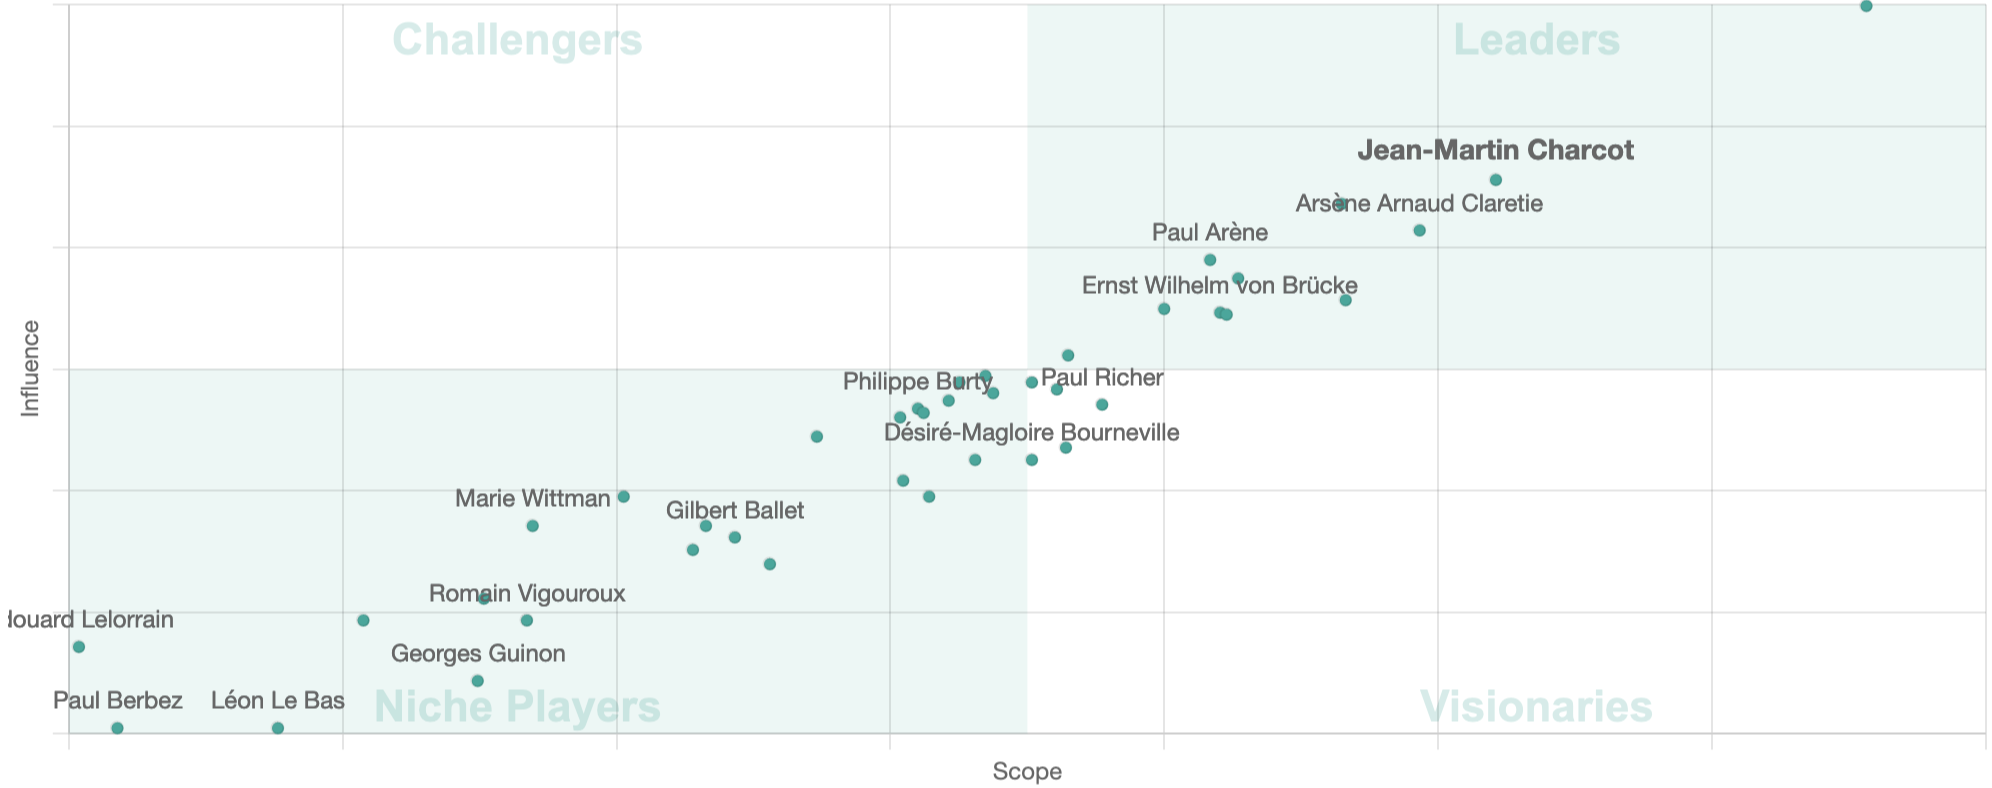
\includegraphics[width=1\textwidth]{img/analyse_quadrant.png}
	\caption[Positionnement de l'entité \texttt{Jean-Martin Charcot} au sein de son domaine et comparaison avec les entités les plus similaires à lui \textit{via} une analyse de quadrant de l'outil Rankingdom.]{Positionnement de l'entité \texttt{Jean-Martin Charcot} au sein de son domaine et comparaison avec les entités les plus similaires à lui \textit{via} une analyse de quadrant de l'outil Rankingdom\protect\footnotemark{.}}
	% Pour raison de visibilité, l'image originale a été agrandie, ce qui a entraîné le rapprochement des années sur l'axe de l'abscisse.
	\label{fig:analyse_quadrant}
\end{figure}

\footnotetext{\url{https://www.rankingdom.org/entity/Q20710?search=jean-martin+charcot}. Le domaine dans lequel Charcot figure est relativement large, y compris les figures du domaine médical (p. ex. Bourneville), mais aussi littéraire (Arsène Arnaud Claretie).}

\bigskip
L'impact de Charcot peut également être visualisé à l'aide de Rankingdom à travers le graphique qui apporte une dimension temporelle (figure \ref{fig:impact_temporel}). Il s'agit notamment de la cumulation temporelle de son impact, où l'on peut observer qu'il s'étend sur la période 1856--1994. 

\begin{figure}[h]
	\centering
	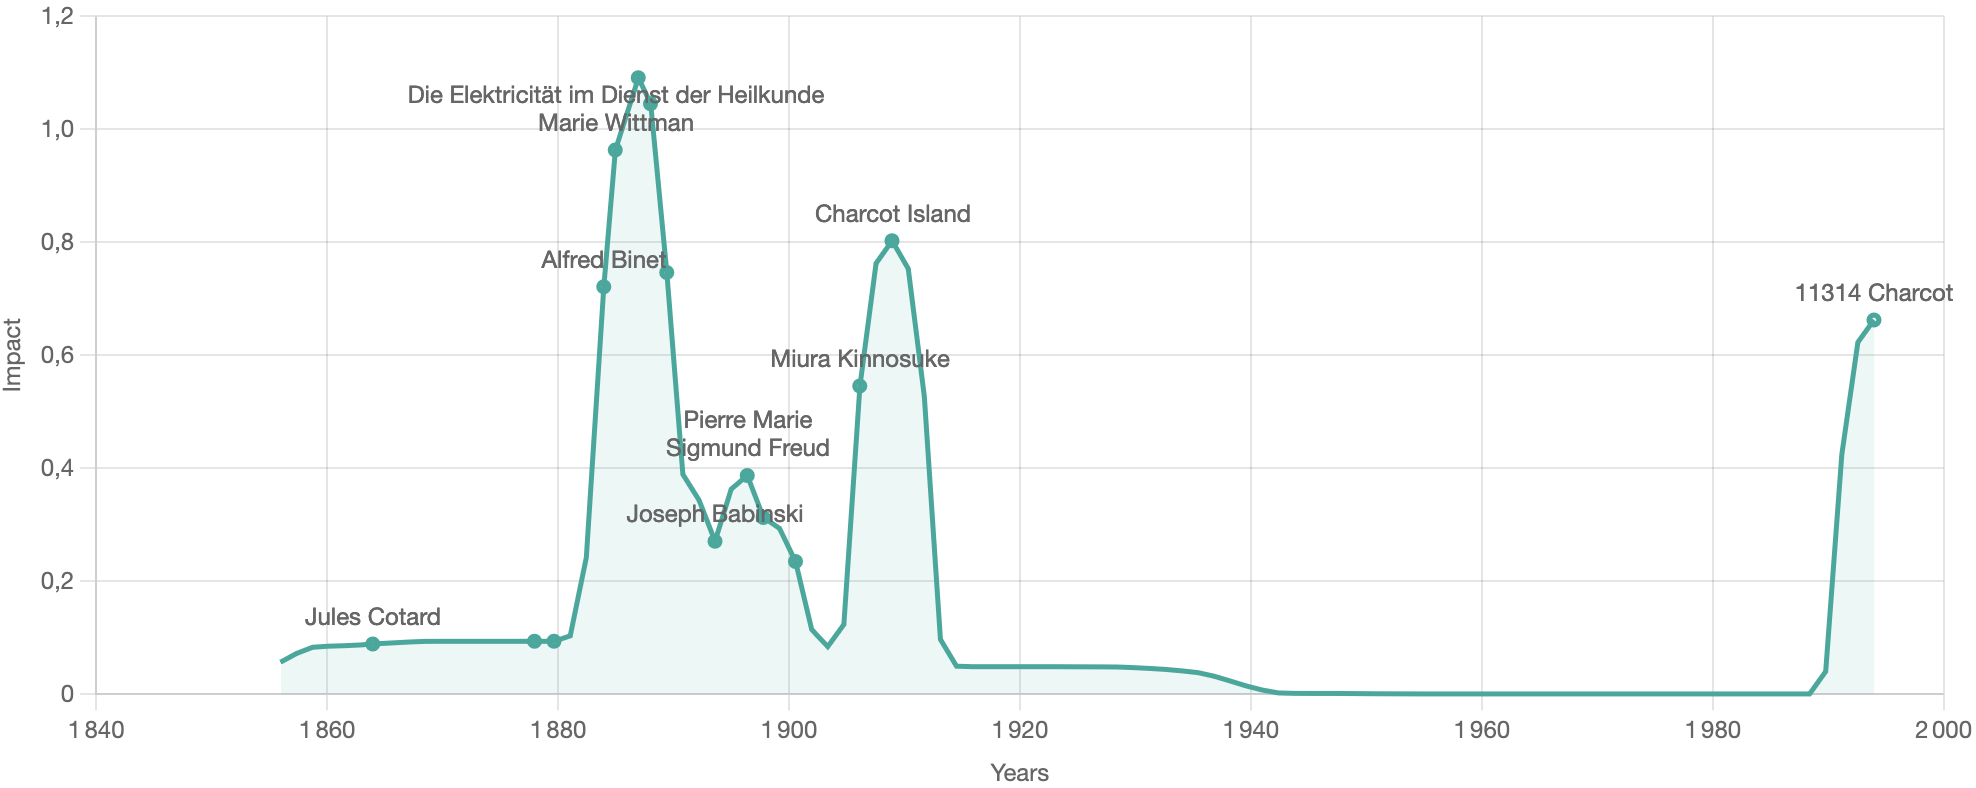
\includegraphics[width=1\textwidth]{img/impact_temporel.png}
	\caption[Analyse temporelle de l'impact de l'entité \texttt{Jean-Martin Charcot} à l'aide de l'outil Rankingdom.]{Analyse temporelle de l'impact de l'entité \texttt{Jean-Martin Charcot} à l'aide de l'outil Rankingdom\protect\footnotemark{.}}
	% Pour raison de visibilité, l'image originale a été agrandie, ce qui a entraîné le rapprochement des années sur l'axe de l'abscisse.
	\label{fig:impact_temporel}
\end{figure}

\footnotetext{\url{https://www.rankingdom.org/entity/Q20710?search=jean-martin+charcot}.}

Enfin, il est également possible de lister les entités impactées, comprenant les personnes (p. ex. Sigmund Freud), les notions médicales (SEP) ou bien les entités géographiques afférentes (Île Charcot).

\label{sect:sota}
\begin{table}[h]
	\centering
	\begin{tabularx}{\textwidth}{|>{\centering\arraybackslash}p{3.5cm}|>{\centering\arraybackslash}X|>{\centering\arraybackslash}X|}
		\hline
		Type & Titre &  \\
		\hline
	\end{tabularx}
\end{table}

\hl{SotA, cadre théorique de la thèse}

\url{https://docs.google.com/document/d/1eoW3mDiHYB9vrPtG-5pdPuaUAAUJpWDa/edit\#heading=h.gjdgxs}


Étant donné l'importance des travaux de Charcot et ses contributions dans le domaine de la neurologie et au-delà, nous souhaitons explorer la notion de la circulation des savoirs au prisme du numérique à travers son impact. Avant d'aborder la question d'opérationnalisation de son impact, nous tenons d'abord à décortiquer les mécanismes à l'origine des circulations des savoirs à grande échelle, ainsi que de définir la notion d'un \og{}concept\fg{} pouvant véhiculer les informations importantes concernant les circulations en question. 





%La section \ref{concept} élabore les différentes approches pour définir plus globalement la notion des concepts historiques qui nous orienteront vers une définition des concepts médicaux en particulier. \smalltodo{pont}



\section{Repérage des termes scientifiques dans un corpus numérique}
\label{termes}
Si nous nous limitons aux théories abordées jusqu'à maintenant, nous pouvons considérer que les concepts médicaux de Charcot ont eu le rôle des vecteurs de la crise conceptuelle, ce qui représentait une forme de \textit{Sattelzeit} dans le domaine de la médecine. Autrement dit, ces concepts ont été détournés de leurs sens initiaux ayant une apparence formelle neutre (descriptions des pathologies), vers ceux exerçant un certain impact sur la communauté scientifique que nous souhaitons mesurer informatiquement. Néanmoins, l'analyse numérique des concepts n'est pas une tâche triviale non plus, car tous les logiciels ne traitent pas des textes de la même manière. D'après \citeauthor{silberztein2022linguistic} (\citeyear{silberztein2022linguistic}, p.~2), les logiciels comme \textsc{TXM}\footnote{\url{https://txm.gitpages.huma-num.fr/textometrie/}}, Sketch Engine\footnote{\url{https://www.sketchengine.eu/}} ou \textsc{IR}a\textsc{M}u\textsc{T}e\textsc{Q}\footnote{\url{http://www.iramuteq.org/}} traitent les documents comme des \textit{séquences de formes graphiques} (dans notre cas, les séquences \og{}hystérie\fg{} et \og{}arthrite déformante\fg{} seraient composées d'une et de deux formes graphiques, respectivement). Ces formes sont définies comme les séquences contiguës de caractères alphabétiques délimités par des non-lettres ou les délimiteurs, qui peuvent être considérées comme des informations potentiellement  pertinentes pour une étude. D'autres logiciels, comme \textsc{N}oo\textsc{J}\footnote{\url{https://nooj.univ-fcomte.fr/}}, peuvent traiter ces séquences comme les \textit{unités linguistiques atomiques}, quel que soit le nombre de formes graphiques \citep[pp.~2-3]{silberztein2022linguistic}. Ainsi, l'unité linguistique atomique \og{}hystérie\fg{} serait recensée dans un dictionnaire des entrées lexicales simples (\textsc{DELAS}), tandis que \og{}arthrite déformante\fg{} ferait partie du dictionnaire des entrées lexicales composées (\textsc{DELAC})\footnote{Ce principe est repris lors du développement du logiciel Unitex \url{https://unitexgramlab.org/fr}.}.

Afin d'extraire automatiquement les concepts scientifiques, nous les opérationnalisons comme des \textit{termes} scientifiques. On en trouve une analogie proche dans la distinction terminologique relevée par \citeauthor{saussure1915} (\citeyear{saussure1915}, pp.~74-75) entre un \textit{signifié} (p. ex. le concept d'un arbre dans notre système cognitif) et un \textit{signifiant} (mot, parole, pictograme désignant un arbre) qui consitue un \textit{signe} (référent, un arbre réel). Les termes sont des expressions textuelles et unités sémantiques qui désignent des concepts dans un domaine d'expertise spécifique. Par conséquent, la tâche d'extraction des concepts peut donc être formalisée comme un problème d'extraction de la terminologie (angl. \textit{automatic text extraction -- \textsc{ATE}}), dont les enjeux appartiennent au domaine de l'extraction d'information (angl. \textit{information retrieval}), et plus largement, à celui du \textsc{TAL}. L'\textsc{ATE} a pour objectif de faciliter l'identification manuelle des termes à partir de corpus spécifiques à un domaine en fournissant une liste de termes candidats \citep[p.~1]{tran2023recent}. Jusqu'à maintenant, trois grandes méthodes d'extraction de la terminologie ont été recensées dans la littérature : linguistique, statistique et la méthode basée sur les apprentissages machine et profond (angl. \textit{machine learning} et \textit{deep learning}, respectivement).
\hl{À FAIRE}
\begin{itemize}
	\item TermoStat\footnote{https://termostat.ling.umontreal.ca/doc\_termostat/doc\_termostat.html} \citep{drouin2003} : termes simples vs. complexes nominaux ; à base de règles ; limite de corpus : 30 Mo + connexion échouée ou phénomène de bottleneck ; extraction des POS
	\item extraction terminologique \texttt{TermSuite}\footnote{\url{https://termsuite.github.io/}} \citep{cram2016terminology} : scalable, \texttt{TreeTagger}
	\item approche linguistique : besoin d'expert du domaine, analyse syntaxique, POS tagging qui a ses limitations, ne peut pas mesurer la pertinence du terme
	\item approche statistique, pas besoin d'expert du domaine, mesure de pertinence : \textit{termhood} et \textit{unithood} \citep[pp.~6-7]{kageura1996} vs. fréquence
	\item approche apprentissage machine / profond : \citep{tran2023recent}
	\item Pour nous, concept scientifique est opérationnalisé comme un terme scientifique.
\end{itemize}




%Motasem :
%revenir sur les concepts de l'index
%comment identifier les concepts médicaux dans les textes ? 
%regarder les fréquences des concepts médicaux
%quelles formes ?
%comment les identifier dans un texte ?
%lire la proposition de Motasem sur les anecdotes et celle de Glenn sur les embeddings dynamiques
%\textsc{ATISHS} : outil pour les HN 
%faire les stats à partir de la liste des concepts -- index (cooccurrences, pattern matching etc.) : qu'est-ce qui marche et marche pas ?

\textbf{Comment définir les concepts scientifiques du point de vue du TAL / analyse du corpus ? concepts, termes et mots-clés}



%Le mot \og{}concept\fg{} est un terme générique qui renvoie à un grand nombre de théories provenant de divers domaines de pensée, sans qu'il en existe une qui soit exhaustive et universellement acceptée.



%En revanche, selon les linguistes, un concept a une structure double, constituée du sens linguistique et culturel.
%%dont linguistique (générale, cognitive, psycholinguistique, ethnolinguistique), philosophie, métaphysique ou mathématiques
%Sa couche intérieure est constituée du noyau étymologique sur lequel repose ensuite la couche périphérique qui hérite les éléments formés par la culture, les traditions et les expériences humaines
%%\foreignlanguage{russian}{(Степанов, \citeyear{stepanov2007}}). 
%\footnote{En linguoculturologie, on retrouve le terme \og{}concept linguo-culturel\fg{} qui reflète cette nature double du concept.}. Il peut être exprimé par de différentes éléments du langage, soit : lexèmes, idiomes, collocations, phrases ou textes entiers \citep[p.~5]{nemickiene2011concept}. 

Dans le domaine du traitement automatique des langues (\textsc{TAL}), le terme \og concept \fg{} peut s'apparenter à celui des \og entités nommées \fg{}, comme en témoignent les recherches sur l'extraction automatique de la terminologie biomédicale (\citealp{jolly2024exploring,navarro2023clinical}). Un concept d'un domaine de connaissance peut faire partie d'un thésaurus, liste organisée de termes contrôlés et normalisés, auquel cas le concept est appelé \og descripteur \fg{}. \citep[p.~16]{RENNESSON202015}.

Un exemple de ce phénomène est le terme \textsc{mot}, qui véhicule une réalité particulière appartenant à chaque langue (\citeauthor{mounin1968clefs} \citeyear{mounin1968clefs}, p. 65). 

Nous n'entendons pas le terme \textsc{concept} dans le sens de Saussure,.... signe = concept (signifié) + image acoustique (signifiant)

Même si l'on reprend la description de Saussure qui considère le mot comme \og une image acoustique associé à un concept \fg{}, nous nous heurtons ensuite au problème de la définition du terme \textit{concept}. Le structuralisme linguistique de Bloomfield souligne ce point, en ajoutant que les linguistes ne sont pas outillés pour démêler complètement ce réseau complexe. Ce structuraliste poursuit en disant que le langage peut en effet être perçu comme une abstraction construite à partir de nos connaissances sur celui-ci, mais qu'il faut \og décrire d'abord le fonctionnement de cet instrument de communication \fg{} et expliquer comment nous (dé)construisons les énoncés en tant que locuteurs ou auditeurs (\citeauthor{mounin1968clefs} \citeyear{mounin1968clefs}, pp. 94-95).

\begin{itemize}
	\item ok, et c'est quoi le concept en linguistique (de Saussure) et en analyse du discours
	\item nous différencions des concepts des \og{}figements linguistiques\fg{} \citep{bezancon2023}
\end{itemize}



Dans le souci de différencier ces notions à travers les disciplines citées, nous présentons ci-dessous quelques-uns de leurs traits discriminatoires qui ne prétendent être ni exhaustifs ni limitatifs :

\begin{table}[h]
	\centering
	\begin{tabular}{|l|l|l|l|}
		\hline
		& \multicolumn{1}{c|}{\begin{tabular}[c]{@{}c@{}}Philosophie\\ Épistémologie\end{tabular}} & \multicolumn{1}{c|}{Linguistique} & \multicolumn{1}{c|}{TAL} \\ \hline
		\textsc{Idée}    & objet de connaissance                                                                                          \citep[p.~261]{Lecourt1999} &                                   &                          \\ \hline
		\textsc{Concept} & représentation de l'objet de connaissance \citep[p.~261]{Lecourt1999}                                                                                      \\ \hline 
		\textsc{Signifié} &  \citep[p.~27]{astolfi2008chapitre}                                                                                      \\ \hline
		\textsc{Signifiant} &    mode de représentation des signifiés \citep[p.~27]{astolfi2008chapitre}                              &                          \\ \hline
		\textsc{Terme}   &                                                                                          &                                   &                          \\ \hline
		\textsc{Mot} &                                                                                          &                                   &                          \\ \hline
		\textsc{Mot-clé} &                                                                                          &                                   &                          \\ \hline
	\end{tabular}
\end{table}

\begin{itemize}
	\item \textbf{Proposer de formaliser la définition du concept (identifiables dans un corpus), mots clés ? Embeddings ? —>} 
	\item nous nous appuyons sur une approximation d'un tel concept, car la tâche d'automatisation et d'implémentation dans l'optique computationnelle enlève forcément quelques traits de concepts abordés dans ce chapitre
\end{itemize}





%\section{Études numériques des circulations culturelles}
\label{circulations}


%Les humanités numériques au service de l'analyse des circulations culturelles
%
%Comment définir une circulation du point de vue de l'analyse du texte ? de la linguistique computationnelle (TAL) ?

%\minitoc

